\documentclass[12pt]{article}
 \usepackage[margin=1in]{geometry} 
\usepackage{amsmath,amsthm,amssymb,amsfonts}
\usepackage{graphicx}
\usepackage{array}
\newcolumntype{P}[1]{>{\centering\arraybackslash}p{#1}}
\newcommand{\N}{\mathbb{N}}
\newcommand{\Z}{\mathbb{Z}}
 
\newenvironment{problem}[2][Problem]{\begin{trivlist}
\item[\hskip \labelsep {\bfseries #1}\hskip \labelsep {\bfseries #2.}]}{\end{trivlist}}
%If you want to title your bold things something different just make another thing exactly like this but replace "problem" with the name of the thing you want, like theorem or lemma or whatever
 
\begin{document}
 
%\renewcommand{\qedsymbol}{\filledbox}
%Good resources for looking up how to do stuff:
%Binary operators: http://www.access2science.com/latex/Binary.html
%General help: http://en.wikibooks.org/wiki/LaTeX/Mathematics
%Or just google stuff
 
\title{Homework-1}
\author{N Dinesh Reddy \\ dnarapur@andrew.cmu.edu }


\maketitle
\section{Representing the world with visual worlds}
\begin{problem}{1.0}
The filters help to convert an image to a meaningful representation. We elaborate on properties captured by each filter below:\\
\underline{\textbf{Filters 1-5:}} The displayed filters are \textbf{gaussian} filters. These filters help in capturing the information in the surrounding pixels. They are a weighted sum of the intensities of the surrounding pixels with a decreasing weight based on the distance from the center pixel. These filters extract the color information of the neighbourhood into the pixel.\\
\underline{\textbf{Filters 6-10:}} These filters represent the \textbf{laplacian of Gaussian} filters. These filters are used to capture rapid changes in the intensity of color of the image. These filters belong to the derivative class of filters. At a sharp edge between two regions, the response will be zero far away from the edge and on the the edge, positive to one side and negative on the other side. This filter gives the highest value to corners and decreasing value to lighter edges.\\
\underline{\textbf{Filters 11-15:}} These filters can be named as directional filters. They are produced by apply a directional bias to a Gaussian filter. The following filters capture variation in appearance in horizontal direction. The filter gives higher response when left neighbourhood posses higher intensify to the right neighbourhood of the center pixel. This can be attributed because of the mask having negative values on the right hand side of the image.\\
\underline{\textbf{Filter 16-20:}} The filters in this category are very similar to the earlier filter category but with the variation that they are vertical filters. They capture the variation in the vertical direction and give higher response when pixels in the upper region have higher value to the lower pixels. 

\end{problem}

 \begin{problem}{1.1} We now apply the filters to an LAB image and display the results for two images below:
 
\begin{figure}
  \centering
  \begin{minipage}[b]{0.45\textwidth}
    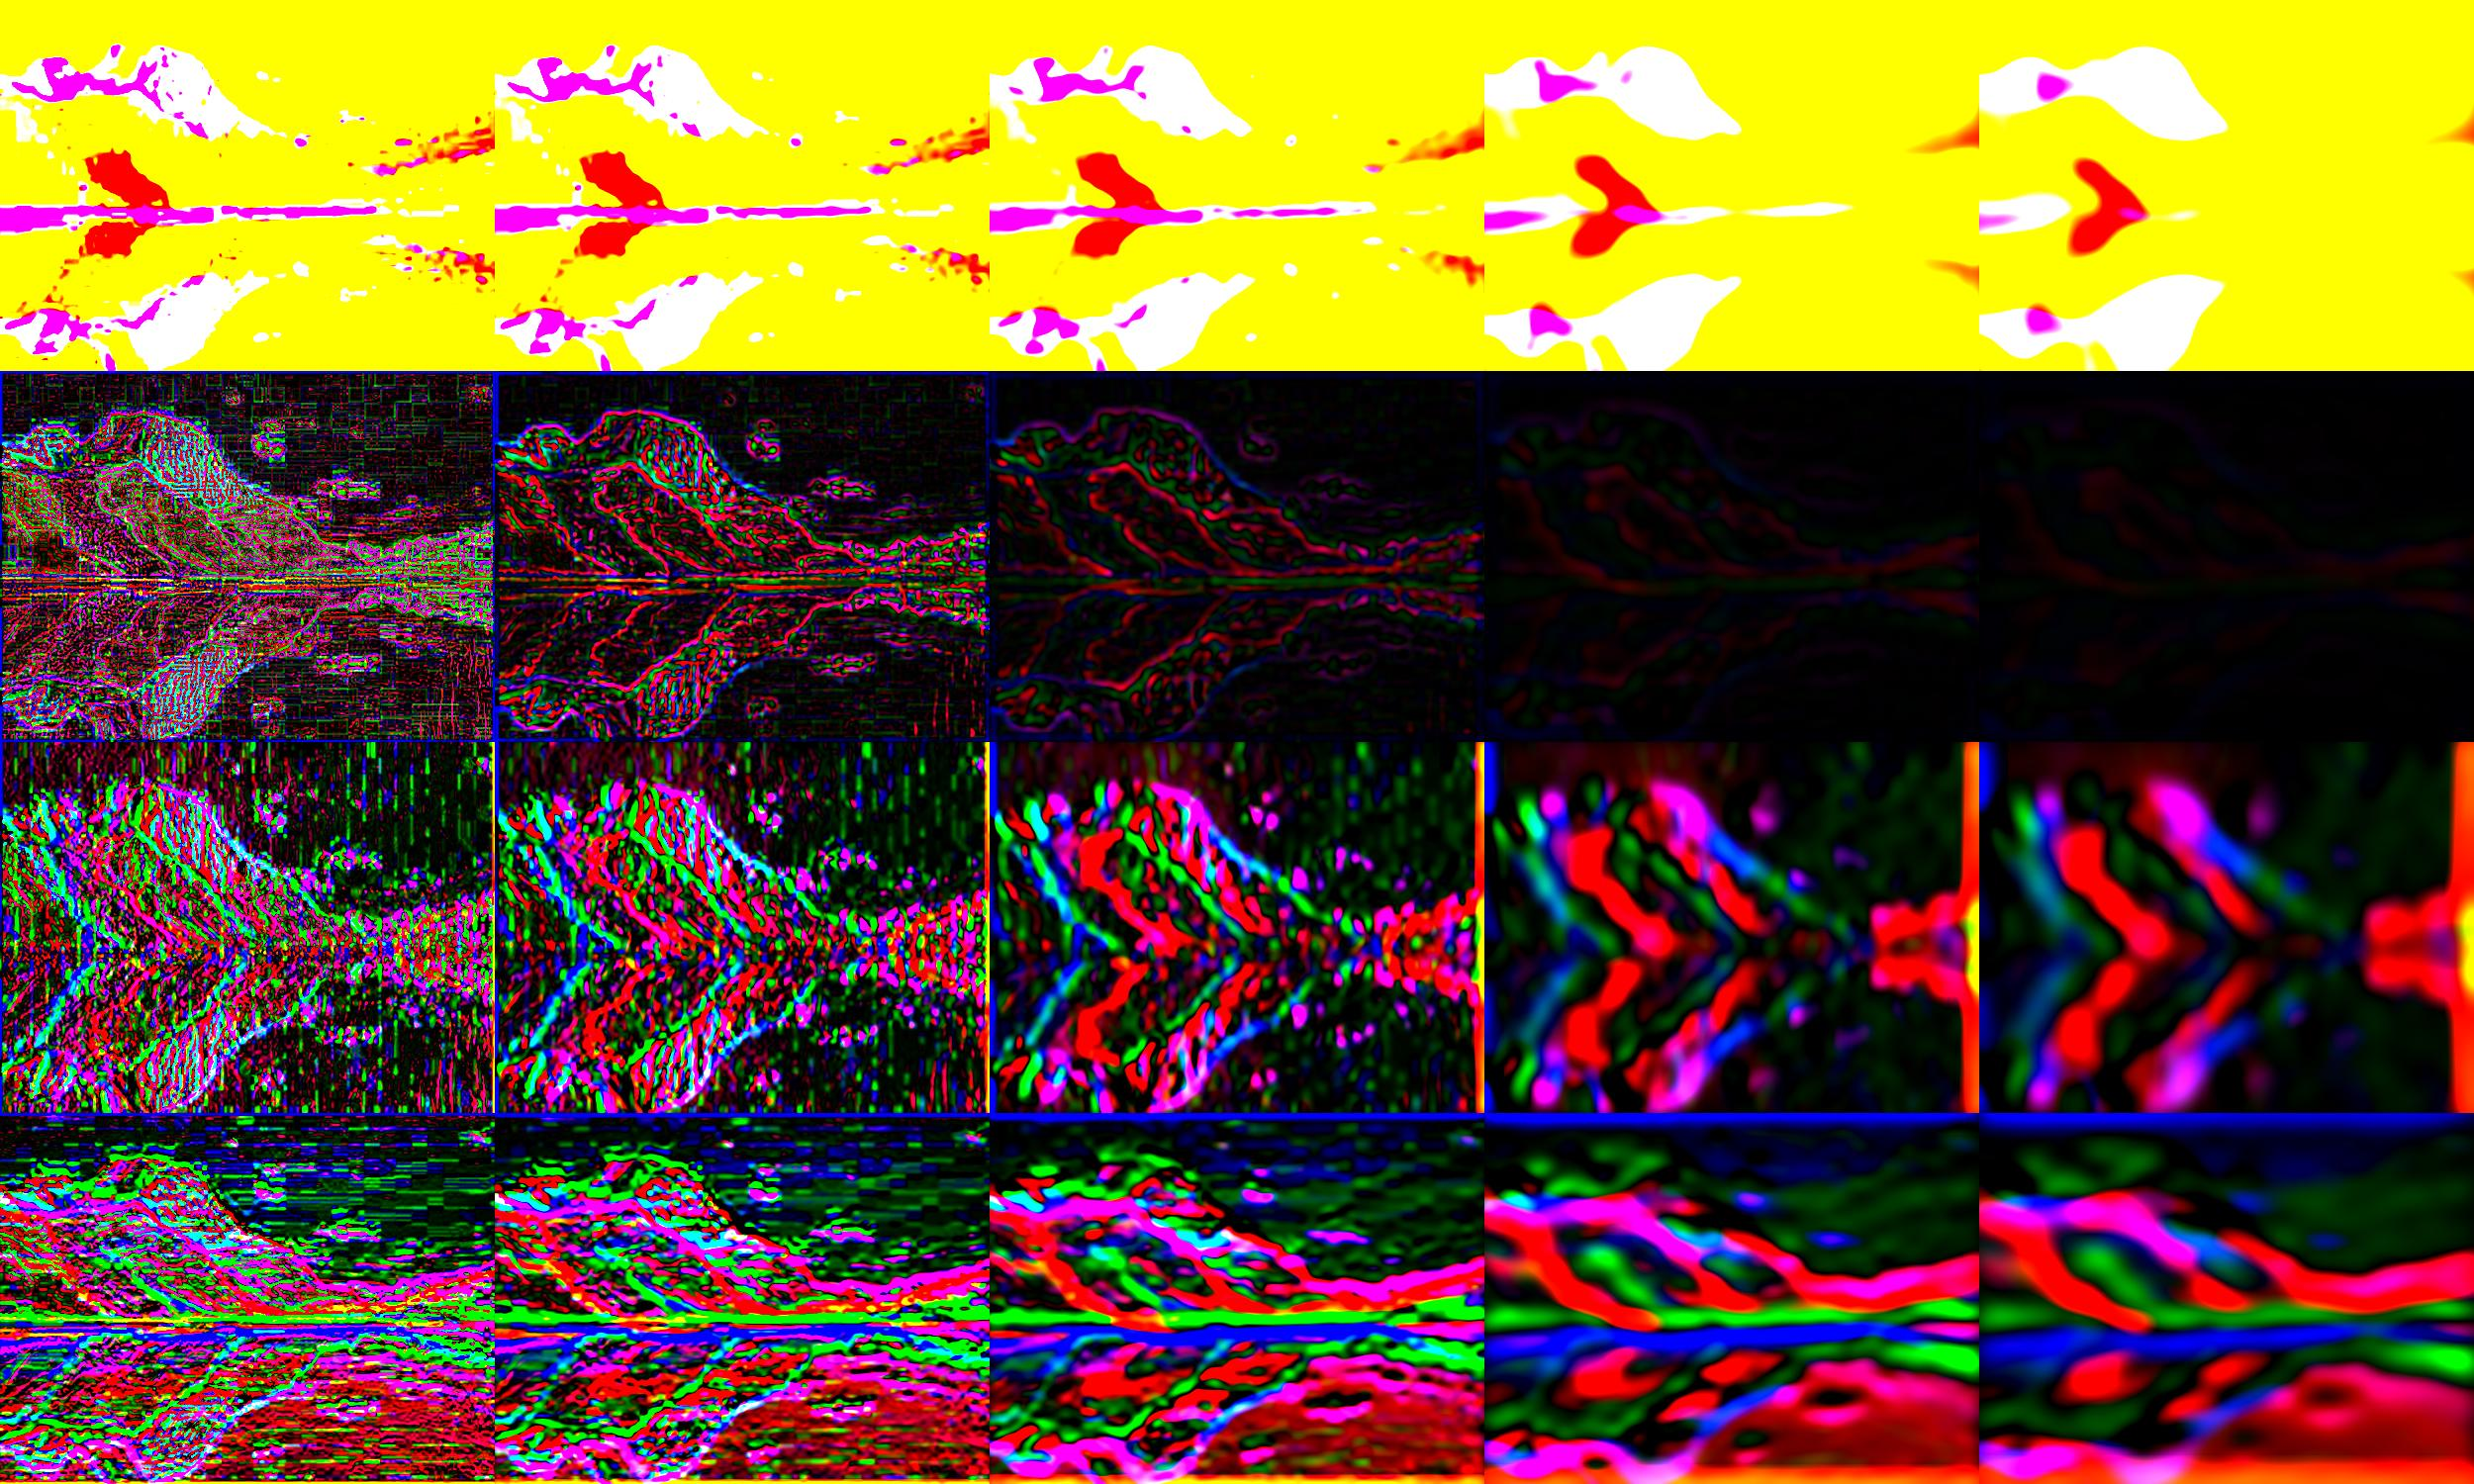
\includegraphics[width=\textwidth]{images/1}
  \end{minipage}
  \begin{minipage}[b]{0.35\textwidth}
    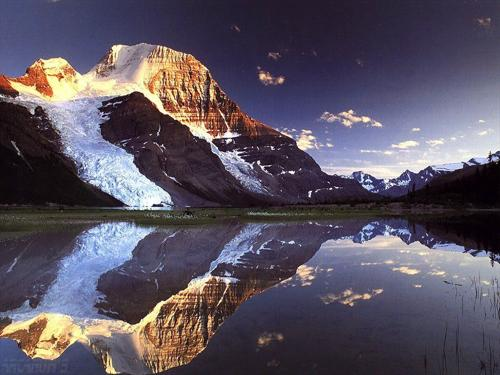
\includegraphics[width=\textwidth]{images/2_o}
  \end{minipage}
\end{figure}

\begin{figure}
  \centering
  \begin{minipage}[b]{0.45\textwidth}
    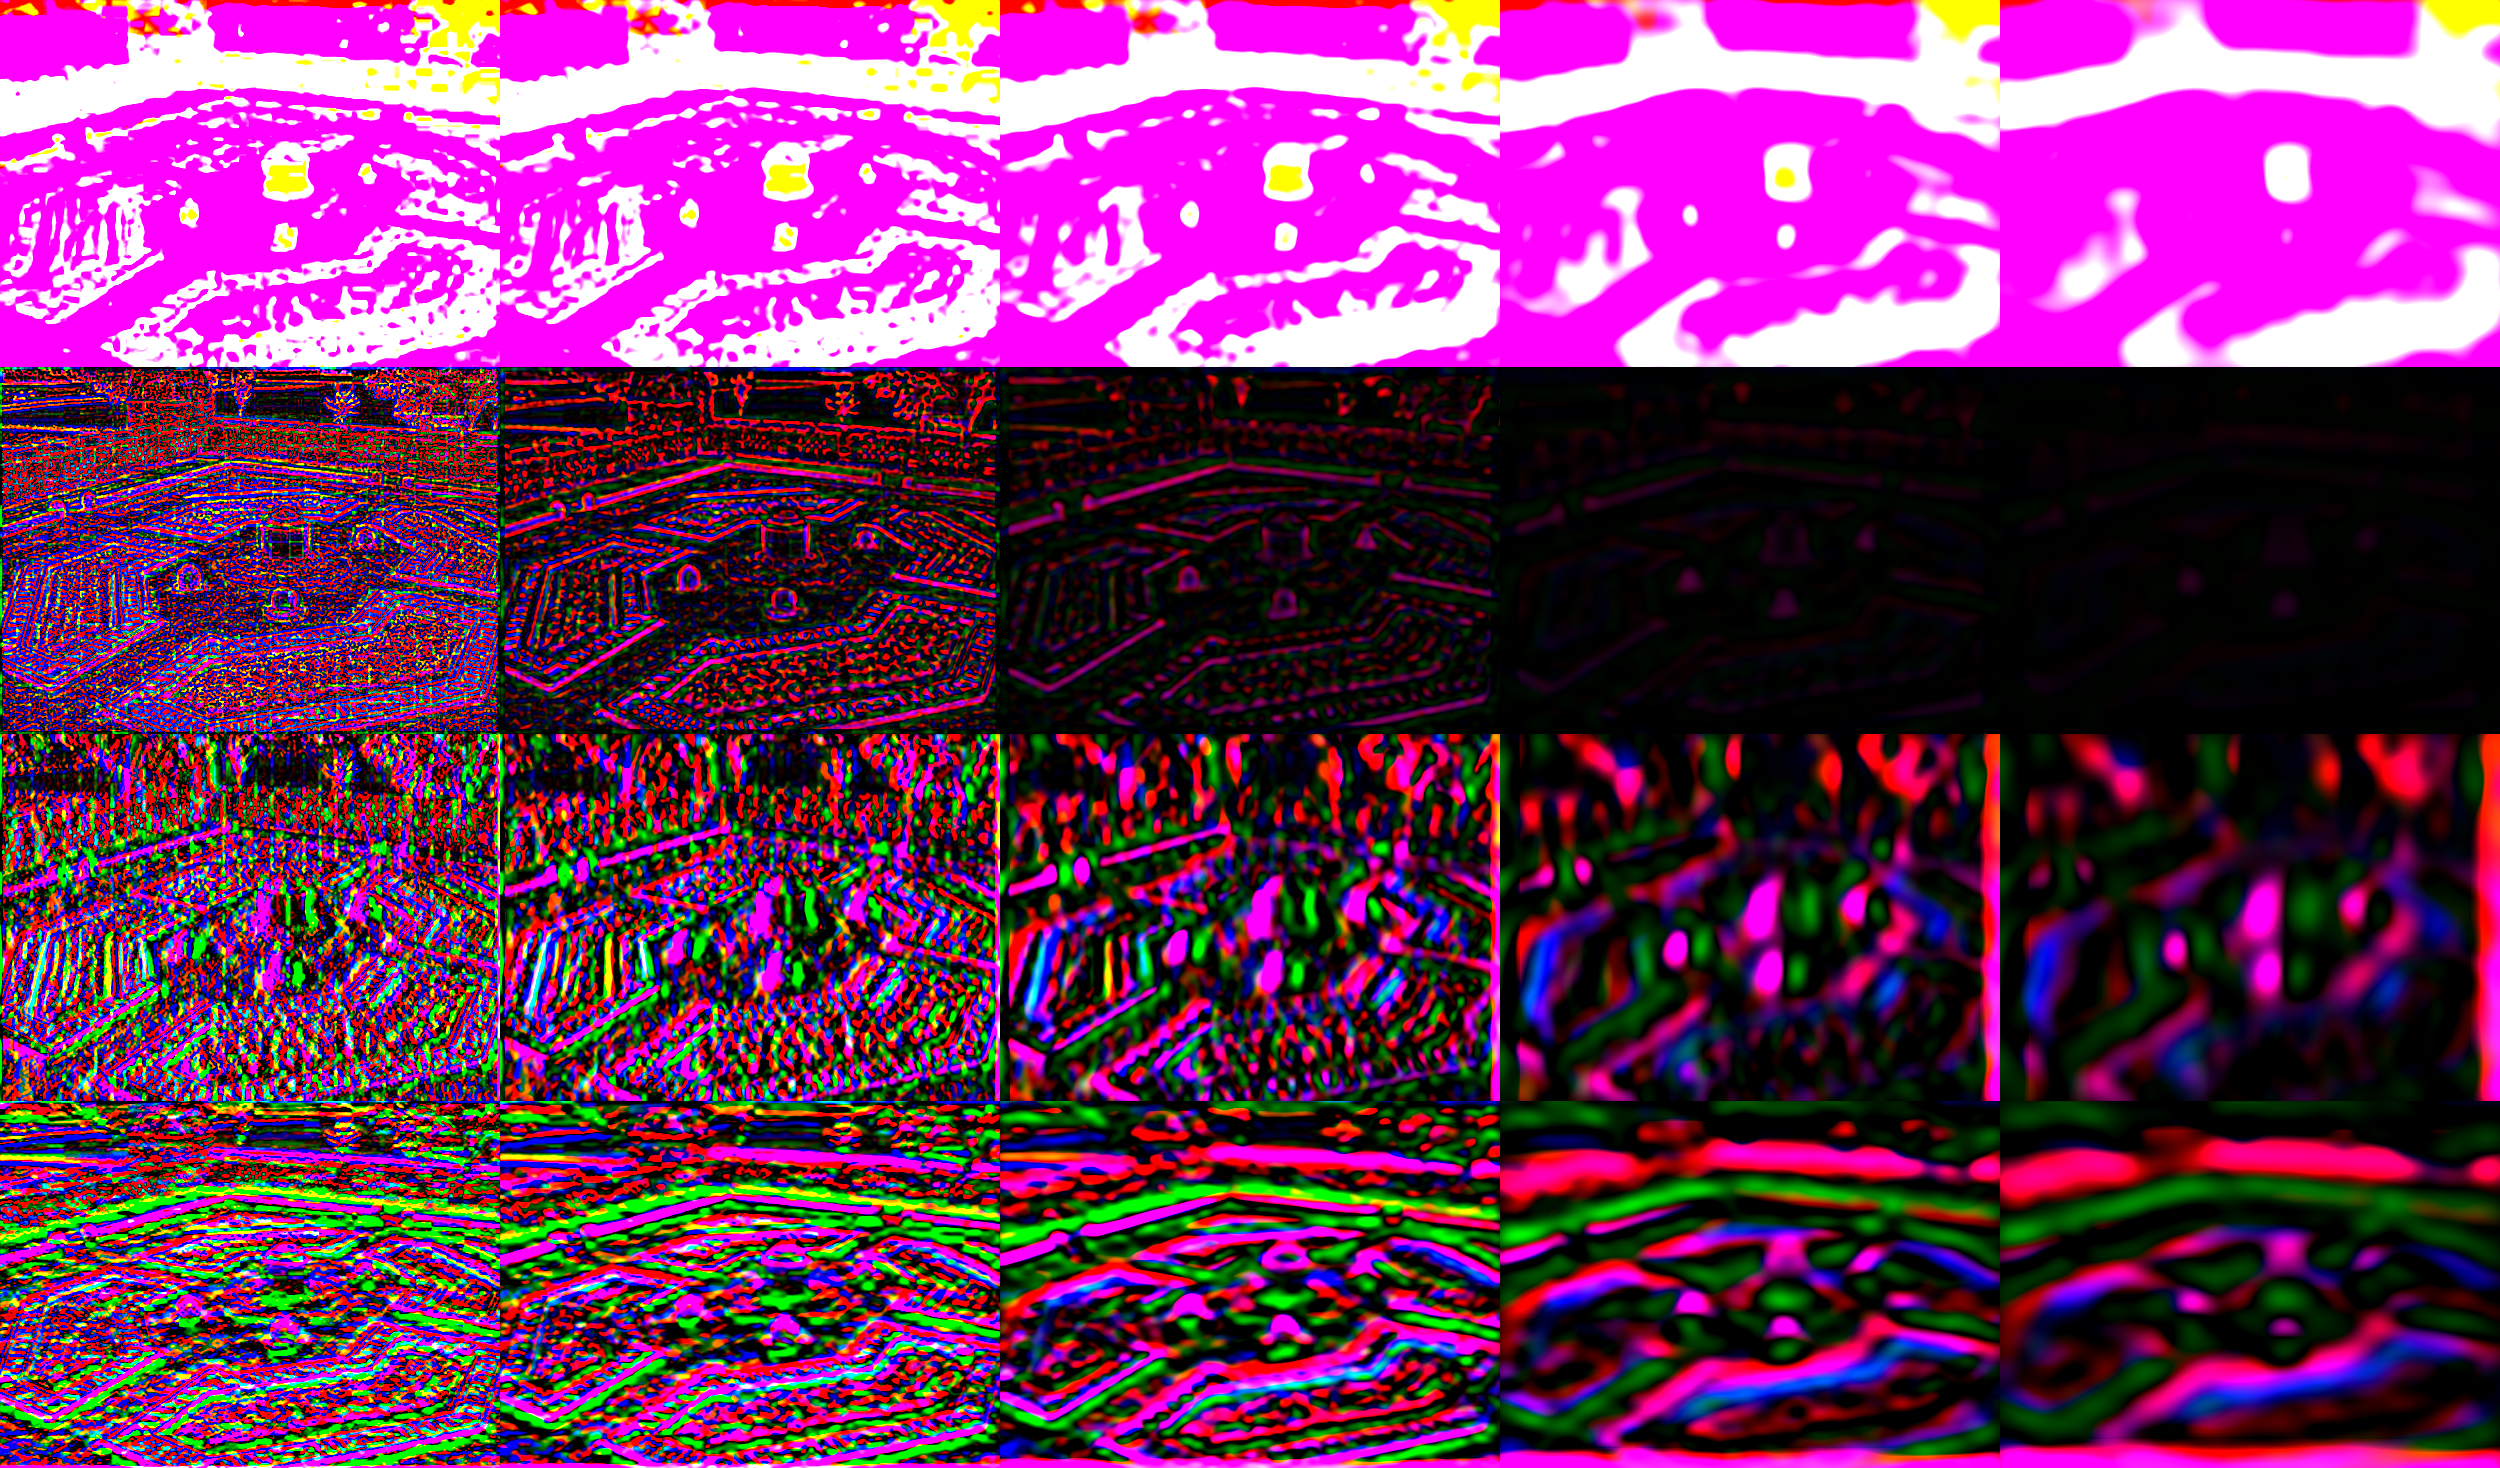
\includegraphics[width=\textwidth]{images/2}
  \end{minipage}
  \begin{minipage}[b]{0.35\textwidth}
    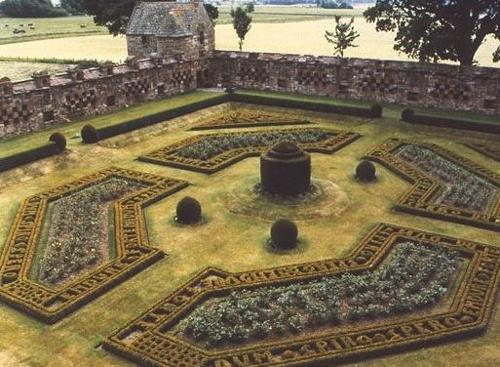
\includegraphics[width=\textwidth]{images/1_o}
  \end{minipage}
\end{figure} 

%\begin{figure}[]
 % \centering
%  \begin{minipage}[b]{0.5\textwidth}
%    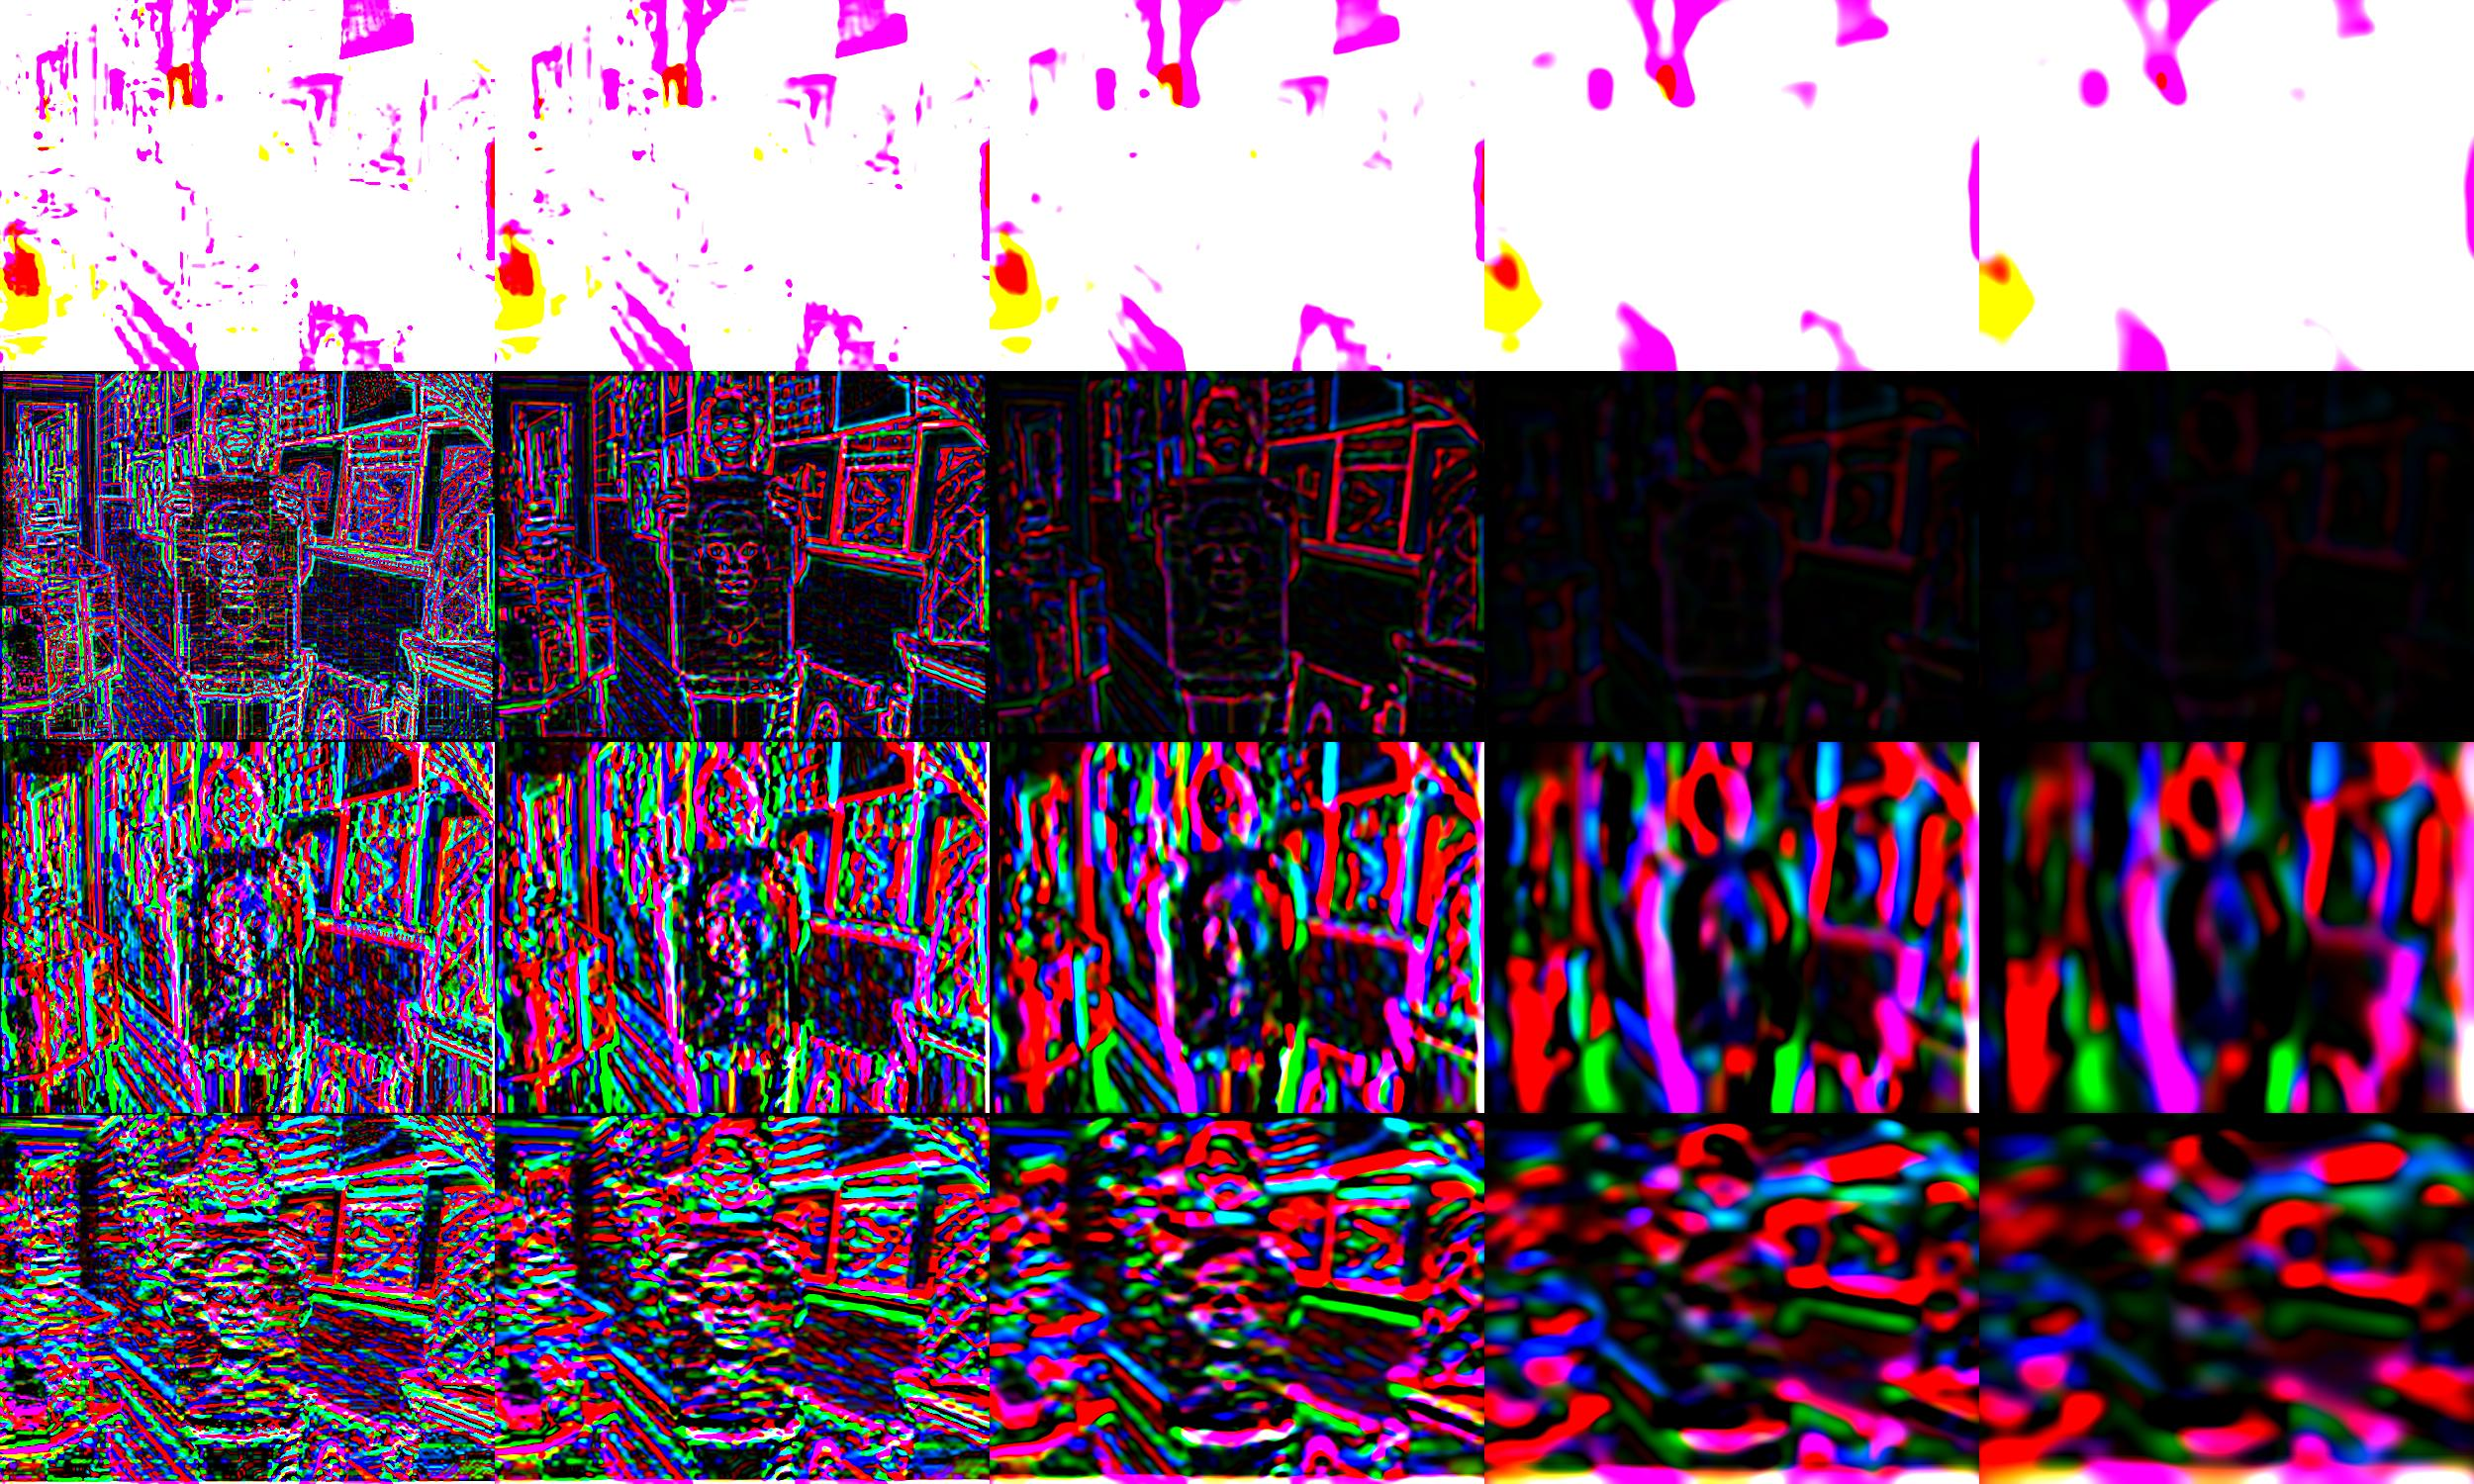
\includegraphics[width=\textwidth]{images/3_o}
%  \end{minipage}
%  \begin{minipage}[b]{0.4\textwidth}
%    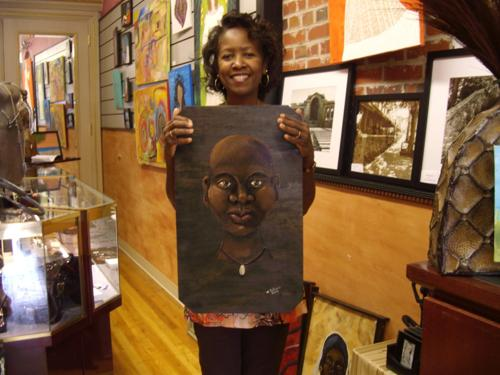
\includegraphics[width=\textwidth]{images/3}
%  \end{minipage}
%\end{figure} 
 
 \end{problem}

\newpage
\begin{problem}{1.3}
We compute the wordmap and display the results for 3 images from the icecate category of the dataset. For all the experiments we have used K = 200 and alpha = 100:

\begin{table}[htb]

\begin{tabular}{c c c}
   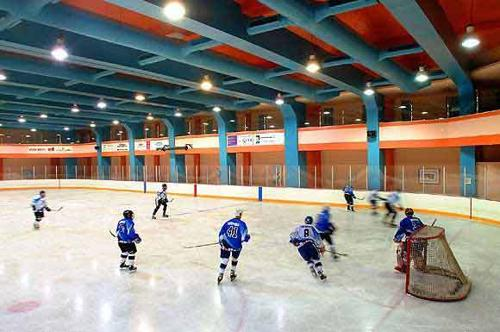
\includegraphics[width=55mm,height=37mm]{images/4_o} &
   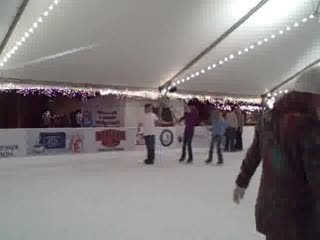
\includegraphics[width=55mm,height=37mm]{images/5_o} &
   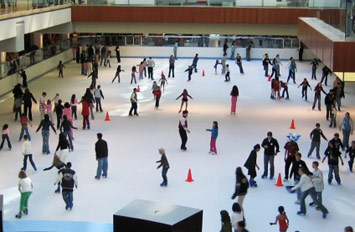
\includegraphics[width=55mm,height=37mm]{images/6_o}\\
   
   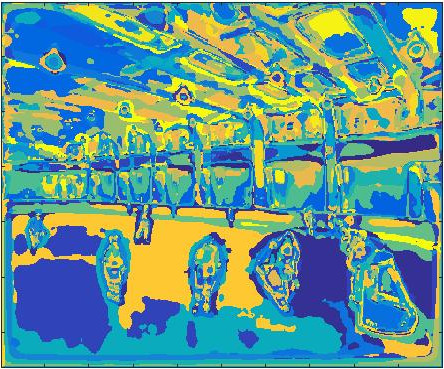
\includegraphics[width=55mm,height=37mm]{images/4} &
   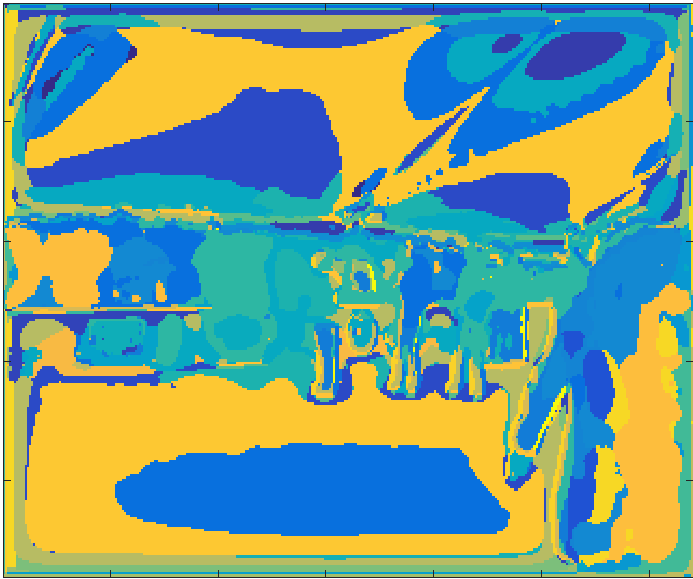
\includegraphics[width=55mm,height=37mm]{images/5} &
   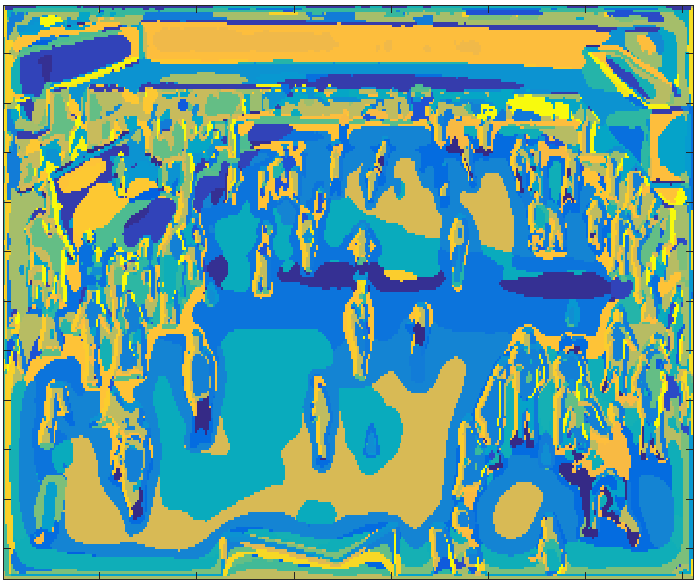
\includegraphics[width=55mm,height=37mm]{images/6}\\
\end{tabular}

\end{table}

\end{problem}
\newpage

\begin{problem}{2.5}
The accuracy of the algorithm comes out to be 54.37\% when the K=200 and alpha = 100 is taking to compute the visual words. the confusion matrix is displayed in table \ref{tab:1} for all the classes. 

\begin{table}


\begin{tabular}{ |p{1.9cm} | P{1.35cm} | P{1.4cm}|  P{1.4cm}|  P{1.4cm} | P{1.4cm}  | P{1.4cm} | P{1.4cm} | P{1.4cm} |}
\hline
 & art gallery &  computer & garden & ice skating & library & mountain & ocean & tennis\\
\hline
art gallery & \textbf{11} & 0 & 0 & 4 & 4 & 0 & 0 & 1\\
computer & 3 & \textbf{8} & 0 & 6 & 2 & 1 & 0 & 0\\
garden & 0 & 0 & \textbf{19} & 0 & 1 & 0 & 0 & 0\\
ice skating & 0 & 3 & 0  & \textbf{16} & 0 & 0 & 0 & 1\\
library    & 6 & 5 & 0 & 1 & \textbf{8} & 0 & 0 & 0\\
mountain   &  1 & 1 & 5 & 0 & 2 & \textbf{9} & 2 & 0\\
ocean    & 2 & 2 & 0 & 2 & 1 & 2 & \textbf{8} & 3\\
tennis & 1 & 5 & 1 & 2 & 1 & 2 & 0 & \textbf{8}\\
\hline


\end{tabular}
\caption{'Confusion matrix for the sample data'}
\label{tab:1}
\end{table}
\end{problem}
\begin{problem}{2.6}
Some of the classes which are tough to classify using the bag-of-words implementation areas can be seen from the confusion matrix are:\\
a) computer room\\
b) library \\
c) ice skating\\

lets try to discuss each failure case. The computer room has a lot of clutter in the image for it to be classified into a specific indoor category. As can be seen from the confusion matrix most of the computer room test images are classified as ice skating or library. This is because of the visual words computed for computer has wide variation in color and locations. This has resulted in classification of the computer lass across all other classes. This justifies the fact that a computer room has too much variation for a easy classification compared to the other classes.  

The library class faces similar problems to the computer room class, where the structure of the indoor scene and wide variation in image colors is causing the miss classification of the library to other similar classes like art gallery and room. To improve the accuracy for such situations of indoor scenes, one of the method can be to increase the number of pyramid levels. The intuition behind this is, scenes like computer room have larger objects and lesser variation within a smaller window compared to art gallery and library which contain smaller objects.

The other class which we are seeing a high misclassification accuracy is for the ice skating category. As can be seen from the confusion matrix the ice skating class has wide spread distribution of wrong classification into nearly all classes. this can be attributed to the fact that among the dataset this class is the only category which has both a uniform plane surface with cluttered humans skating in the field. This leads to the wrong classification of this category into both cluttered environments like computer room, art gallery and classes with uniform texture like tennis court and ocean. 
\end{problem}
\newpage
\begin{problem}{2.7}
To look at improving the accuracy of the current algorithm the first set of experiments conducted are computing accuracy versus the number of pyramid levels. As shown in the figure \ref{fig:acc} we fix all other parameters for the algorithm and vary the number of pyramid levels in the spacial matching algorithm as expected with increase in the spacial subdivisions the accuracy of the algorithm improves. We get an accuracy of 56.8750\% for pyramid level of 4.

\begin{figure}[t]
\begin{center}
	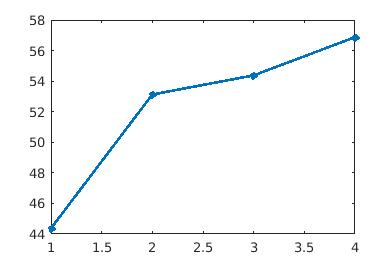
\includegraphics[width=55mm]{images/check}\\
\end{center}
\caption{pyramid level vs accuracy plot}
\label{fig:acc}

\end{figure}

To improve the accuracy the second improvement we propose is to apply neural network for the classification task keeping the same feature extraction algorithm. We show the accuracy boast upto 66.25\% using this neural network with the same features used using the histogram kernel matching. We can further improve the accuracy by using more intelligent feature extraction methods and by preprocessing the images. The confusion matrix after applying a two layer fully connected network is shown in table \ref{tab:2}. As you can see the confusion matrix clearly shows an improvement in all the classes and does not have any bias towards specific classes. This can be attributed to the fact that a fully connected layer over the histogram nullifies any local effected which were causing miss classification earlier. We have a used a simple one layer fully connected network with 32 hidden layer values. We have experimented with different layer architectures and have observed over fitting with multiple layers and misclassification with lee hidden layer values. Further improvement in feature extraction schema can improve the accuracy of the algorithm. All the experiments are conducted with K=200 and alpha=100. Experimented varying these parameters to find variation 2-4 percent in accuracy. 

\begin{table}


\begin{tabular}{ |p{1.9cm} | P{1.35cm} | P{1.4cm}|  P{1.4cm}|  P{1.4cm} | P{1.4cm}  | P{1.4cm} | P{1.4cm} | P{1.4cm} |}
\hline
 & art gallery &  computer & garden & ice skating & library & mountain & ocean & tennis\\
\hline
art gallery & \textbf{9} & 2 & 0 & 3 & 5 & 0 & 0 & 1\\
computer & 3 & \textbf{13} & 0 & 3 & 1 & 0 & 0 & 0\\
garden & 0 & 0 & \textbf{18} & 0 & 0 & 1 & 0 & 1\\
ice skating & 3 & 0 & 0  & \textbf{15} & 1 & 0 & 1 & 0\\
library    & 1 & 4 & 0 & 1 & \textbf{14} & 0 & 0 & 0\\
mountain   &  0 & 1 & 2 & 0 & 1 & \textbf{12} & 2 & 2\\
ocean    & 0 & 1 & 0 & 0 & 1 & 3 & \textbf{14} & 1\\
tennis & 1 & 1 & 3 & 0 & 1 & 1 & 2 & \textbf{11}\\
\hline


\end{tabular}
\caption{'Confusion matrix using neural network'}
\label{tab:2}
\end{table}


\end{problem}

\end{document}